\section{Methodology}\label{sec:methodology2}\label{sec:methodology}

The primary objective of this study is to demonstrate that the Graph Attention Network (GAT) model can better imitate the Strong Branching strategy compared to the Graph Convolutional Neural Network.
This section will discuss the techniques and methods used to mimic the Strong Branching strategy with Graph Attention Network(GAT)-based approaches.
The methodology consists of three phases:

\subsection{Data Collection}\label{subsec:data-collection}
Training data is required to train a machine learning model.
For the GAT models to learn, 100,000 Strong Branching examples were collected separately from randomly generated Set Covering instances following Balas and Ho~\cite{balasSetCoveringAlgorithms1980}, randomly generated Combinatorial Auction instances following Leyton-Brown et al.~\cite{leyton-brownUniversalTestSuite2000} and randomly generated Maximum Independent Set instances following the Bergman et al.~\cite{bergmanDecisionDiagramsOptimization2016}.
These three benchmarks were selected due to their characteristics: they pose significant challenges for state-of-the-art solvers while also serving as representative examples of mixed integer programming problems commonly encountered in practical applications.


The dataset was divided into two subsets, with 80\% allocated for training and the remaining 20\% reserved for validation.
This partitioning ensures that the model is trained on the training data while its performance is evaluated on a separate validation set, allowing for a reliable assessment of its generalization capability.
Details of the training and validation dataset can be seen in Table~\ref{tab:gat-training-data}.

\begin{table*}[htb!]
    \centering
    \begin{tabular}{|l c c c|}
        \hline
        \textbf{Problem Type} & \textbf{Set Covering} & \textbf{Combinatorial Auctions} & \textbf{Maximum Independent Set}\\
        \hline
        \textbf{Training Size} & 80,000 samples & 80,000 samples & 80,000 samples\\
        \textbf{Validation Size} & 20,000 samples & 20,000 samples & 20,000 samples\\
        \textbf{Problem Parameters} & 500 rows, 1000 columns & 100 items for 500 bids & 500 nodes\\
        \hline
    \end{tabular}
    \caption{Details of training and validation dataset used by GAT models.}
    \label{tab:gat-training-data}
\end{table*}

To ensure that the collected Strong Branching examples are as independent from each other as possible, the branching strategy used in solving the problems was Pseudocosts Branching with a 95\% probability and Strong Branching with a 5\% probability, as was done in the study by Gasse et al.~\cite{gasseExactCombinatorialOptimization2019}.
For example, as illustrated in Figure~\ref{fig:sample-distribution}, an analysis of the distribution of sampled nodes in the maximum independent set problems reveals that a sufficient number of samples have been collected from various levels of the branch-and-bound tree.
This approach ensured that Strong Branching examples were collected from different nodes of the search tree as much as possible.

\begin{figure}[htb!]
    \centering
    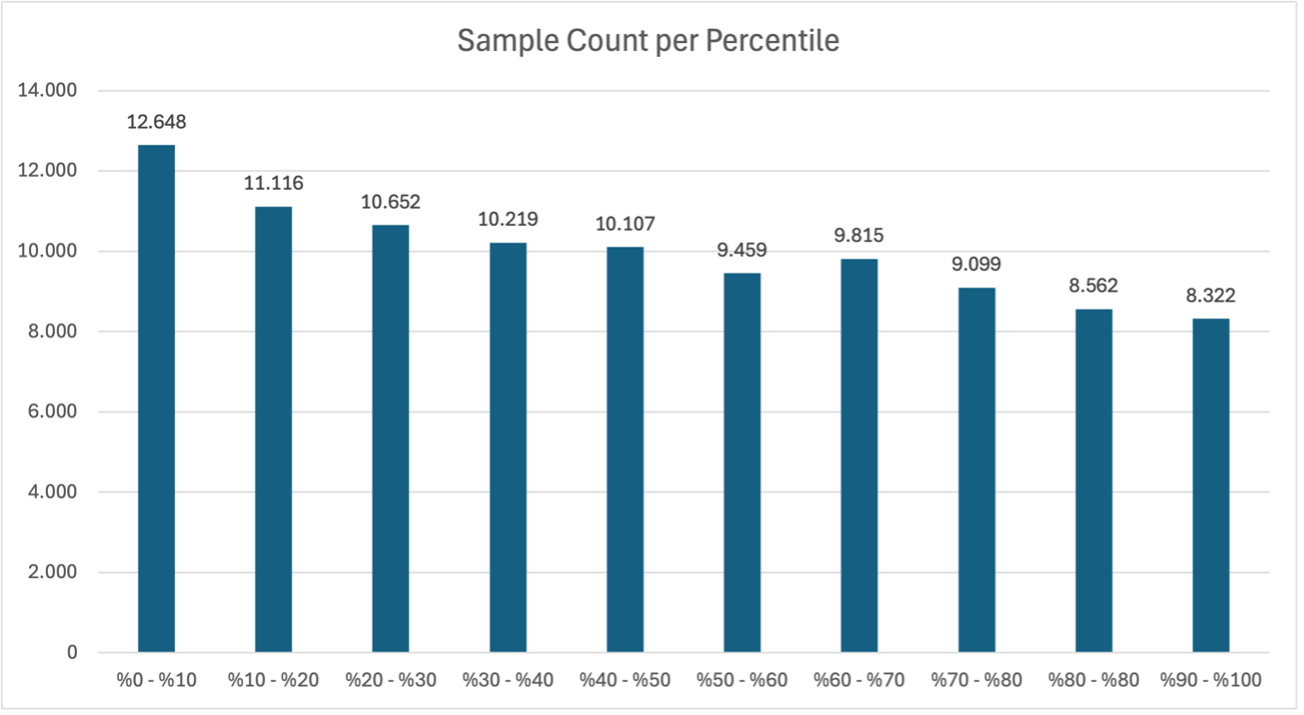
\includegraphics[width=0.45\textwidth]{figures/Sample Distribution}
    \caption{Distribution of 100,000 sampled nodes in the maximum independent set problems according to percentile levels}
    \label{fig:sample-distribution}
\end{figure}


Each training example includes the branching candidate variables, the Strong Branching score calculated by the Strong Branching strategy for the candidate variables, and the variable selected for branching by the Strong Branching strategy.
In addition to the decisions made by the Strong Branching strategy, constraint, variable, and edge features from Table A.0.3, %burası güncellenecek
as well as connectivity data, were also collected, as in the study by Gasse et al.~\cite{gasseExactCombinatorialOptimization2019}.
The reason for considering the features used by Gasse et al.~\cite{gasseExactCombinatorialOptimization2019} is to prevent discrepancies caused by different features when comparing models.
It is believed that this approach would allow for a more accurate comparison of the models.

The generation of random problems, solving the problems using Strong Branching or Pseudocosts Branching, and collecting the training data were all performed using the Python library called ecole~\cite{prouvostEcoleGymlikeLibrary2020a}.


\subsection{Training GAT Models}
The training process was conducted offline.
The GAT models were trained separately for each problem type using 100,000 training examples with the Adam optimizer~\cite{kingmaAdamMethodStochastic2017} and Cross Entropy Loss.
The GAT models trained in this study can be seen in Table~\ref{fig:gat-models} as follows:

\begin{table*}[htb!]
    \centering
    \begin{tabular}{|l c c c c|}
        \hline
        \textbf{Model/Parameters} & \textbf{GAT} & \textbf{MHGAT2} & \textbf{MHGAT4} & \textbf{MHGAT8}\\
        \hline
        \textbf{Number of Convolutions} & 2 & 2 & 2 & 2\\
        \textbf{Number of Attention Heads in First Convolution} & 1 & 2 & 4 & 8\\\
        \textbf{Aggregation Method in First Convolution} & N/A & Concatenate & Concatenate & Concatenate\\
        \textbf{Number of Attention Head in Second Convolution} & 1 & 2 & 2 & 2\\
        \textbf{Aggregation Method in Second Convolution} & N/A & Average & Average & Average\\
        \textbf{Optimizer} & Adam & Adam & Adam & Adam\\
        \textbf{Learning Rate} & 0.001 & 0.001 & 0.001 & 0.001\\
        \textbf{Number of Epochs} & 50 & 50 & 50 & 50\\
        \textbf{Batch Size} & 32 & 32 & 32 & 32\\
        \hline
    \end{tabular}
    \caption{The GAT models trained in this study. “MH” represents “Multi Head”.}
    \label{tab:gat-models}
\end{table*}


The GAT models trained in this study have three main components:

\begin{itemize}
  \item Preprocessing Layers: As in Gasse et al.~\cite{gasseExactCombinatorialOptimization2019}'s study, the variable features and constraint features were transformed into 64-dimensional embeddings using a fully connected 2-layer MLP with ReLU activation function and layer normalization.
  Layer normalization was also applied to the edge features.
  The reason for applying this process to the variable, constraint, and edge features is to enable the model to learn how these features should be updated to achieve optimal performance.
  The model will learn how to transform the variable and constraint features into 64-dimensional embeddings based on the training data.
  \item GAT Layers: TThe key difference between this study and the work of Gasse et al.~\cite{gasseExactCombinatorialOptimization2019} is the use of GAT Convolution layers as convolution layers.
  Unlike Graph Convolutional Neural Networks (GCNN), the Graph Attention Network (GAT) model allows a node's neighbors to have varying degrees of importance for the node itself.
  For this reason, it was hypothesized that the GAT model would better mimic the Strong Branching strategy compared to the GCNN model.
  Therefore, instead of GCNN, two GAT layers were added to the GAT model.
  Design decisions were made when adding the GAT layers to the model to enhance its performance as follows:
  \begin{itemize}
      \item In the GAT convolution operation, the creation of self-loops was disabled.
      This is because MILP problems are represented as bipartite graphs, and self-loops do not hold any meaning in bipartite graphs.
      In the bipartite graphs used, edges exist only between variable and constraint nodes.
      \item After the convolution operation, to retain and preserve the node's own information, the node's own embeddings were concatenated with the embeddings aggregated from neighboring nodes using a learnable skip connection.
      \item Before the concatenation process, the node's own embeddings were passed through a Linear layer.
      The reason for this is to enable the model to learn how to update the node's own embeddings before the concatenation process.
      \item The concatenated embeddings were passed through a ReLU activation function.
  \end{itemize}
  \item Fully Connected MLP: At final stage, the variable embeddings, which have undergone two convolution operations, are passed through a 2-layer MLP.
  A ReLU activation function is used in the first layer.
  A SoftMax activation function is used in the second layer.
  As a result of this process, the 64-dimensional embeddings for each variable are converted into a single dimensional score.
  The model selects the variable with the highest score as the branching variable among branching candidates.
\end{itemize}


The design of the GAT architecture, as well as the training and evaluation processes, were carried out using Python library named PyTorch Geometric~\cite{feyFastGraphRepresentation2019}.
The designed end-to-end GAT architecture is as shown in Figure~\ref{fig:gat}.


\begin{figure*}[htb!]
    \centering
    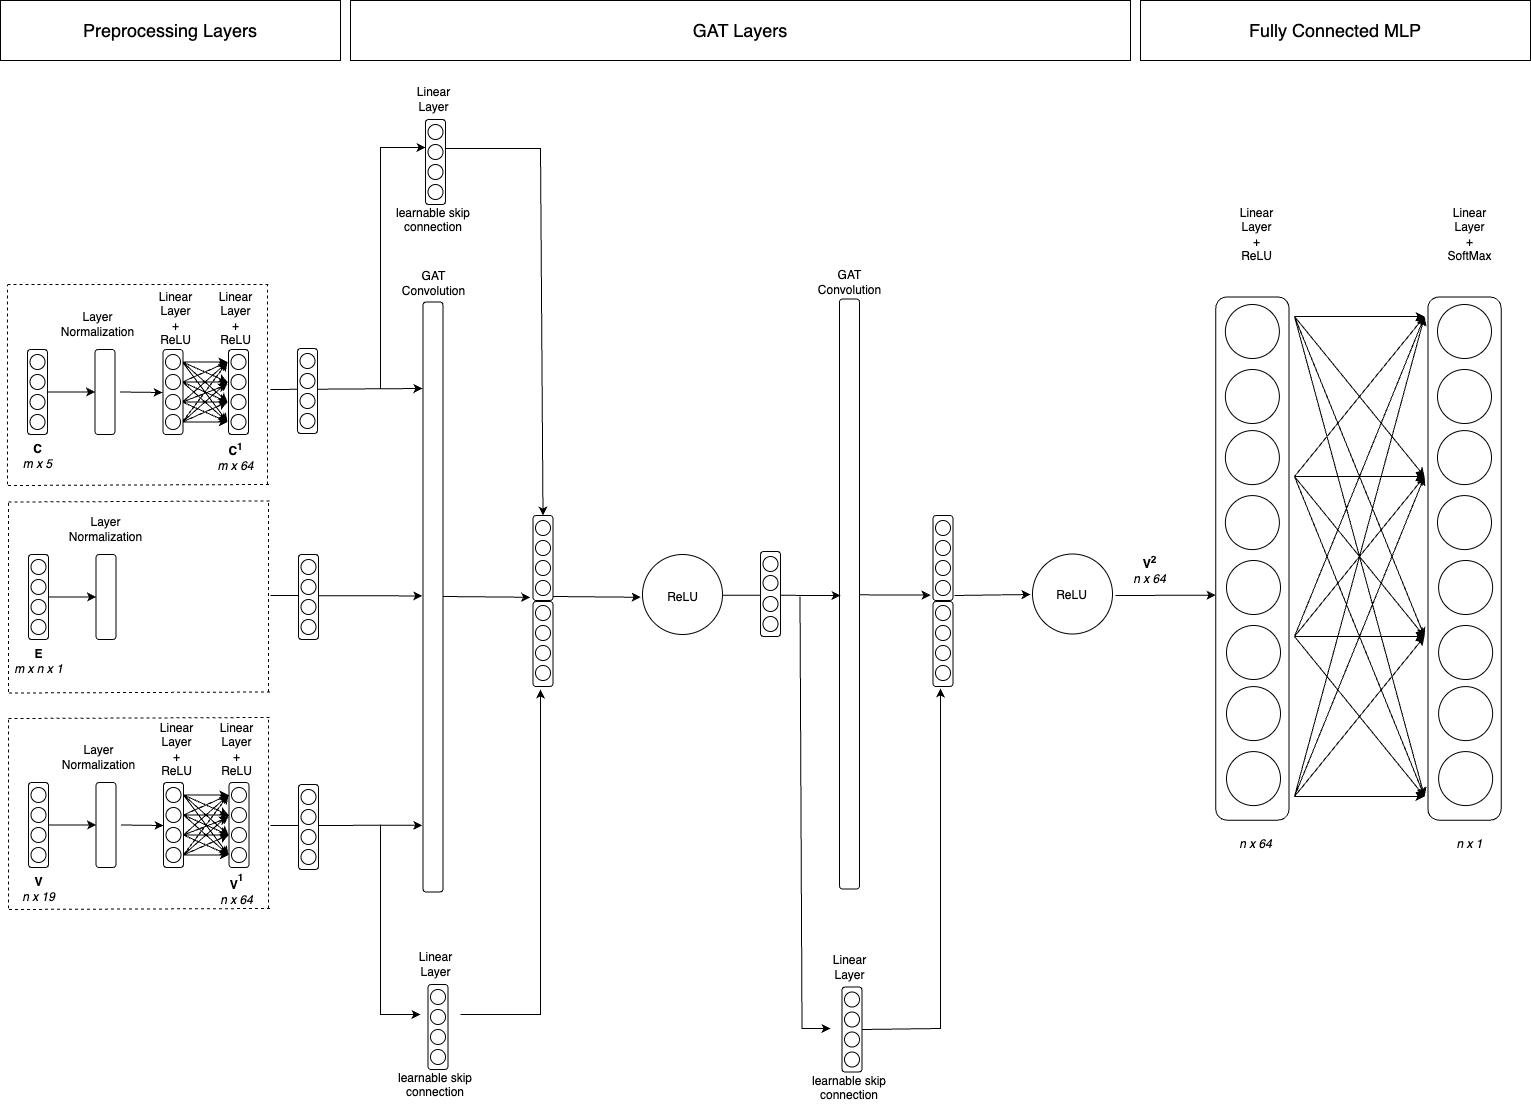
\includegraphics[width=1\textwidth]{figures/GAT}
    \caption{GAT Convolution based GNN architecture.}
    \label{fig:gat}
\end{figure*}

When analyzing the validation accuracy of GAT models on the Set Covering problems, it is evident from Figure~\ref{fig:sc-validation-accuracy} that the MHGAT8 model generally outperforms the other models.
As shown in Table~\ref{tab:sc-validation-accuracy}, the highest validation accuracy at the final epoch was also achieved by the MHGAT8 model.
Based on these findings, the MHGAT8 model was selected for further evaluations on the Set Covering problems, as it demonstrated superior performance in this context.

\begin{table}[htb!]
    \centering
    \begin{tabular}{|l c|}
        \hline
        \textbf{Models} & \textbf{Validation Accuracy}\\
        \hline
        \textbf{GAT} & 0.584\\
        \textbf{MHGAT2} & 0.582\\\
        \textbf{MHGAT4} & 0.582\\
        \textbf{MHGAT8} & \textbf{0.601}\\
        \hline
    \end{tabular}
    \caption{Validation accuracy of GAT models at the final epoch on Set Covering Problems.
    Higher is better, and the best value is in bold.}
    \label{tab:sc-validation-accuracy}
\end{table}

\begin{figure}[htb!]
    \centering
    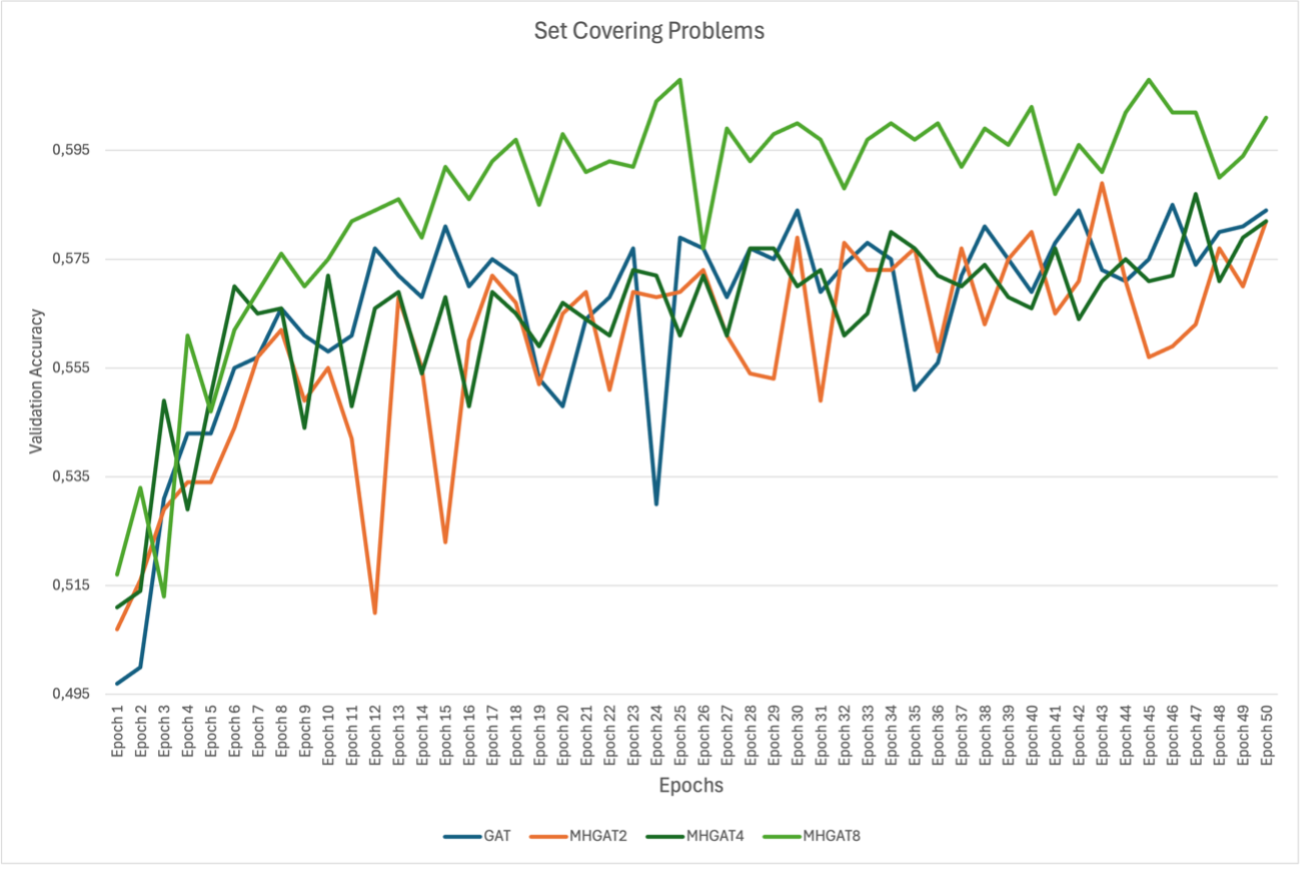
\includegraphics[width=0.45\textwidth]{figures/SC Validation Accuracy}
    \caption{Validation accuracy of GAT models on Set Covering validation dataset.}
    \label{fig:sc-validation-accuracy}
\end{figure}


When analyzing the validation accuracy of GAT models on the Combinatorial Auction problems, it is evident from Figure 4.4~\ref{fig:ca-validation-accuracy} that the MHGAT8 model generally outperforms the other models.
As shown in Table~\ref{tab:ca-validation-accuracy}, the highest validation accuracy at the final epoch was also achieved by the MHGAT8 model.
Based on these findings, the MHGAT8 model was selected for further evaluations on the Combinatorial Auction problems, as it demonstrated superior performance in this context.


\begin{table}[htb!]
    \centering
    \begin{tabular}{|l c|}
        \hline
        \textbf{Models} & \textbf{Validation Accuracy}\\
        \hline
        \textbf{GAT} & 0.541\\
        \textbf{MHGAT2} & 0.542\\
        \textbf{MHGAT4} & 0.564\\
        \textbf{MHGAT8} & \textbf{0.570}\\
        \hline
    \end{tabular}
    \caption{Validation accuracy of GAT models at the final epoch on Combinatorial Auction Problems.
    Higher is better, and the best value is in bold.}
    \label{tab:ca-validation-accuracy}
\end{table}

\begin{figure}[htb!]
    \centering
    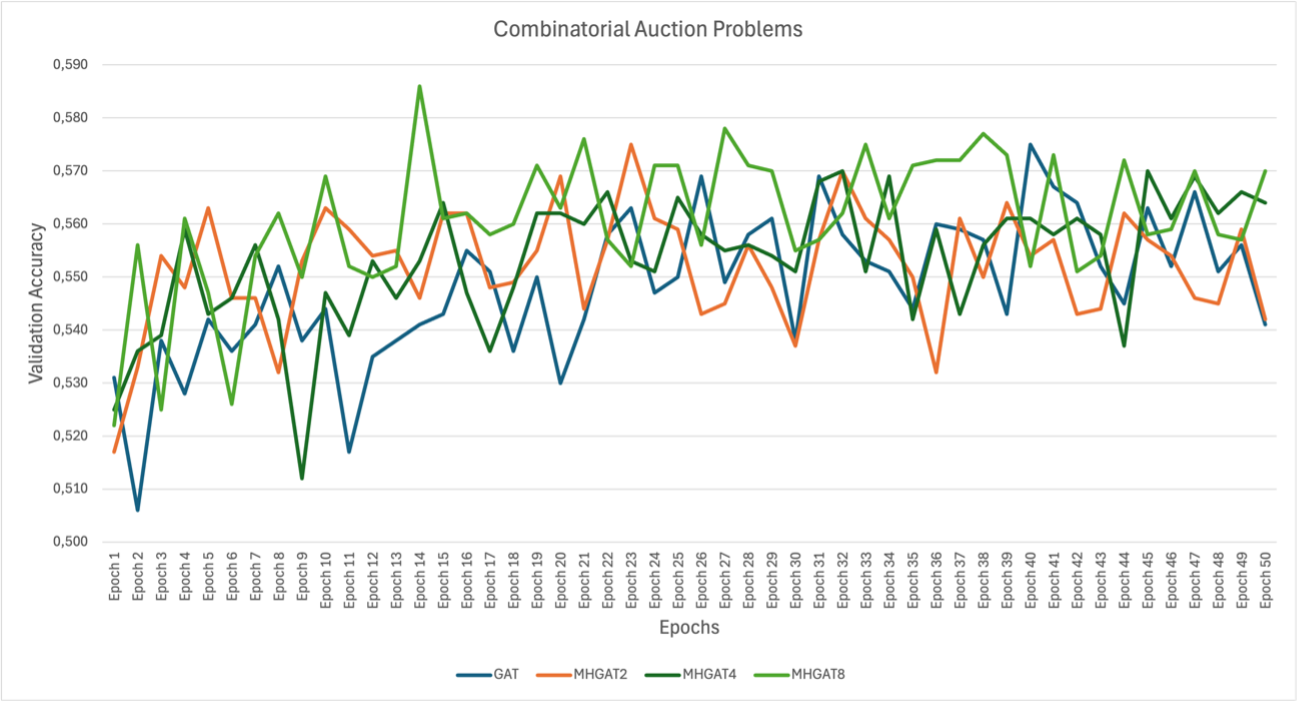
\includegraphics[width=0.45\textwidth]{figures/CA Validation Accuracy}
    \caption{Validation accuracy of GAT models on Combinatorial Auction validation dataset.}
    \label{fig:ca-validation-accuracy}
\end{figure}


When analyzing the validation accuracy of GAT models on the Maximum Independent Set problems, it is evident from Figure 4.5 that the MHGAT8 model generally outperforms the other models.
As shown in Table~\ref{tab:is-validation-accuracy}, the highest validation accuracy at the final epoch was also achieved by the MHGAT8 model.
Based on these findings, the MHGAT8 model was selected for further evaluations on the Maximum Independent Set problems, as it demonstrated superior performance in this context.

\begin{table}[htb!]
    \centering
    \begin{tabular}{|l c|}
        \hline
        \textbf{Models} & \textbf{Validation Accuracy}\\
        \hline
        \textbf{GAT} & 0.522\\
        \textbf{MHGAT2} & 0.526\\
        \textbf{MHGAT4} & 0.533\\
        \textbf{MHGAT8} & \textbf{0.537}\\
        \hline
    \end{tabular}
    \caption{Validation accuracy of GAT models at the final epoch on Maximum Independent Set Problems.
    Higher is better, and the best value is in bold.}
    \label{tab:is-validation-accuracy}
\end{table}

\begin{figure}[htb!]
    \centering
    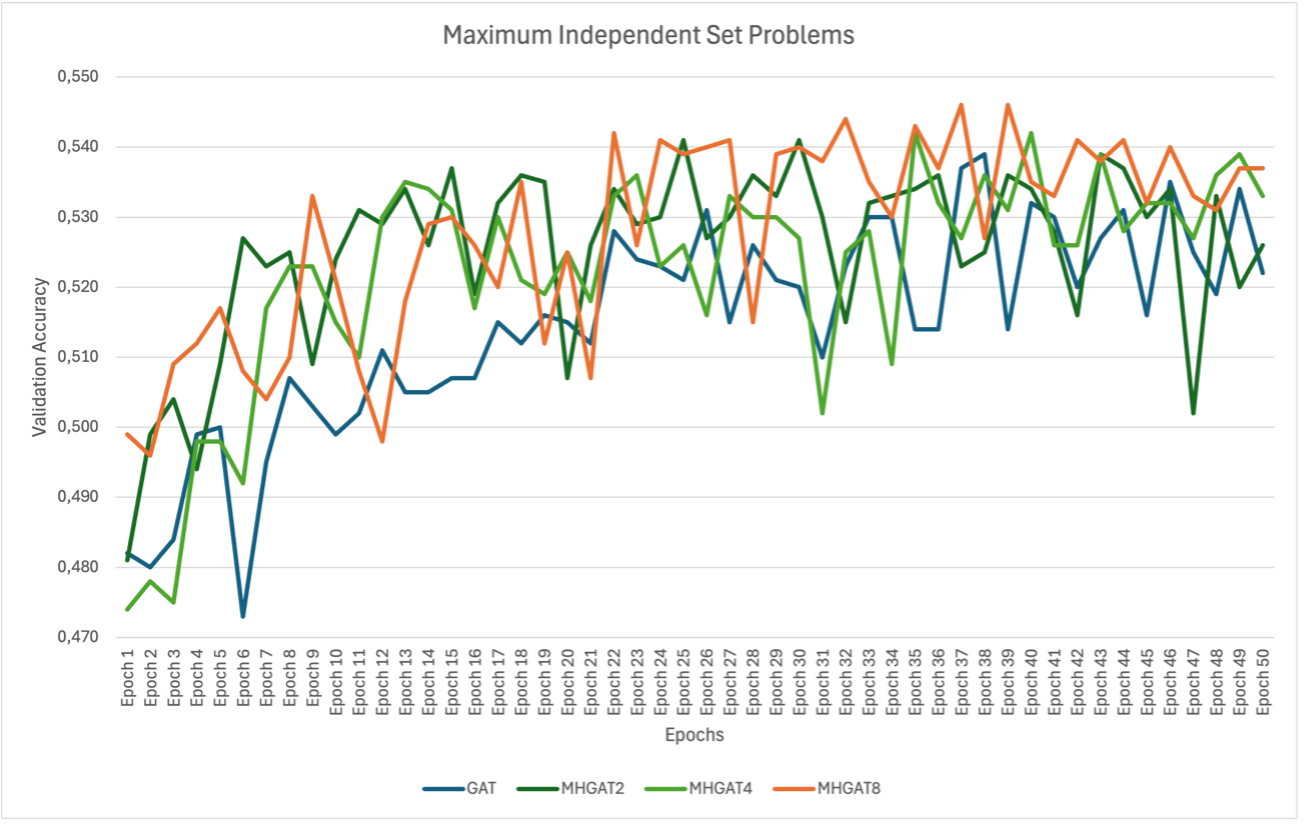
\includegraphics[width=0.45\textwidth]{figures/IS Validation Accuracy}
    \caption{Validation accuracy of GAT models on Maximum Independent Set validation dataset.}
    \label{fig:is-validation-accuracy}
\end{figure}


\subsection{Evaluation}
The GCNN and GAT models were trained using the same set of 100,000 training examples separately for each problem type.
The computations have been performed on Nvidia A100 GPU with 83.5 GB RAM, 40 GB GPU RAM and 235.7 GB Memory.


Throughout the experiments, SCIP 8.0.0 was utilized as the solver, with a time limit set to 1 hour.
Cutting plane generation was restricted to the root node only, and solver restarts were disabled.


At this stage, two separate experiments were conducted.
In the first experiment, 100 randomly generated “Easy” instances of the Set Covering, Combinatorial Auction, and Maximum Independent Set problems were solved individually using the Full Strong Branching (FSB), Most Infeasible Branching (MIB), SCIP’s default brancher Reliability Pseudocost (RPB), GCNN and GAT models.
The problems utilized in this experiment are of the same complexity level as those used for training the models.


In the second experiment, 100 randomly generated “Medium” instances of the Set Covering, Combinatorial Auction and Maximum Independent Set problems were solved individually using the SCIP’s default brancher Reliability Pseudocost (RPB), GCNN and GAT models.
The problems used in this experiment are more complex than those on which the models were trained.
The increase in complexity in Set Covering Problems arises from the growth in the number of constraints, while in Combinatorial Auction Problems, it is attributed to the increase in both the number of constraints and variables.
Experimental results demonstrate that all models solve problems in the “Medium” category with a higher number of nodes and longer computation times compared to problems in the “Easy” category.
The objective is to observe and evaluate the performance of the models when applied to more challenging problem instances, thereby assessing their ability to generalize to higher levels of complexity.
Details of the evaluation dataset can be seen in Table~\ref{tab:gat-evaluation-data}.

\begin{table*}[htb!]
    \centering
    \begin{tabular}{|l c c c|}
        \hline
        \textbf{Problem Type} & \textbf{Set Covering} & \textbf{Combinatorial Auctions} & \textbf{Maximum Independent Set}\\
        \hline
        \textbf{Data Size (Easy)} & 100 instances & 100 instances & 100 instances\\
        \textbf{Problem Parameters (Easy)} & 500 rows, 1000 columns & 100 items for 500 bids & 500 nodes\\
        \textbf{Data Size (Medium)} & 100 instances & 100 instances & 100 instances\\
        \textbf{Problem Parameters (Medium)} & 1000 rows, 1000 columns & 200 items for 1000 bids & 1000 nodes\\
        \hline
    \end{tabular}
    \caption{Details of the evaluation dataset used by GAT models.}
    \label{tab:gat-evaluation-data}
\end{table*}


\subsubsection{Results}
The primary characteristic of the Strong Branching strategy is its ability to minimize the number of nodes in the search tree.
This study aims to demonstrate that the Graph Attention Network (GAT) strategy can better imitate the Strong Branching strategy compared to the Graph Convolutional Neural Network (GCNN).
Consequently, the primary evaluation criterion is the average number of nodes required by the models to solve the problems.


As shown in the Table~\ref{tab:sc-results-easy}, the MHGAT8 model solved the Set Covering problems in the "Easy" category with an average of 0.79\% fewer nodes compared to the GCNN model.
When comparing the models in terms of time, the MHGAT8 model took, on average, 58.02\% longer to solve the problems than the GCNN model.
However, as previously noted, the primary evaluation criterion in these experiments is the average number of nodes.


Another statistic reveals that out of 100 problems, the MHGAT8 model solved 52 problems with fewer nodes, while the GCNN model outperformed in 38 cases.
In 10 problems, both models produced an equal number of nodes.
These results suggest that the MHGAT8 model better imitates the Strong Branching strategy for “Easy” Set Covering problems compared to the GCNN model.


When comparing GCNN and MHGAT8 with other models, as expected, both models were faster than the Full Strong Branching (FSB) model.
However, the FSB model achieved solutions with fewer nodes.
Both GCNN and MHGAT8 outperformed the Most Infeasible Branching (MIB) algorithm in terms of both node count and solution time.
Additionally, while GCNN and MHGAT8 demonstrated better performance than the SCIP’s default brancher Reliability Pseudocost Branching (RPB) algorithm in terms of time, RPB outperformed both models in terms of node count.

\begin{table*}[htb!]
    \centering
    \begin{tabular}{|l c c c c c|}
        \hline
        \textbf{Models} & \textbf{Number of Nodes} & \textbf{Improvement} & \textbf{Time} & \textbf{Improvement} & \textbf{Win}\\
        \hline
        \textbf{FSB} & 13.19 $\pm$ 2.04 & - & 32.16 $\pm$ 3.25 & - & -\\
        \textbf{MIB} & 1,156.5 $\pm$ 5.63 & - & 10.59 $\pm$ 3.09 & - & -\\
        \textbf{RPB} & 47.30 $\pm$ 3.78 & - & 6.27 $\pm$ 1.66 & - & -\\
        \hline
        \textbf{GCNN} & 123.55 $\pm$ 2.79 & - & \textbf{3.79 $\pm$ 1.61} & - & 38/100\\
        \textbf{MHGAT8} & \textbf{122.57 $\pm$ 2.82} & \textcolor{green}{0.79\%} & 5.99 $\pm$ 1.98 & \textcolor{red}{-58.02\%} & \textbf{52/100}\\
        \hline
    \end{tabular}
    \caption{Evaluation results for “Easy” Set Covering problems. “Number of Nodes” and “Time” (in seconds) are shifted geometric means over instances with shifts 10 and 1, respectively.
    A "win" was defined as solving a problem with fewer nodes.
    Best value among GCNN and GAT is in bold.}
    \label{tab:sc-results-easy}
\end{table*}

As shown in the Table~\ref{tab:ca-results-easy}, the MHGAT8 model solved the Combinatorial Auction problems in the "Easy" category with an average of 4.91\% fewer nodes compared to the GCNN model.
When comparing the models in terms of time, the MHGAT8 model took, on average, 6.77\% longer to solve the problems than the GCNN model.
However, as previously noted, the primary evaluation criterion in these experiments is the average number of nodes.


Another statistic reveals that out of 100 problems, the MHGAT8 model solved 55 problems with fewer nodes, while the GCNN model outperformed in 36 cases.
In 9 problems, both models produced an equal number of nodes.
These results suggest that the MHGAT8 model better imitates the Strong Branching strategy for “Easy” Combinatorial Auction problems compared to the GCNN model.


When comparing GCNN and MHGAT8 with other models, as expected, both models were faster than the Full Strong Branching (FSB) model.
However, the FSB model achieved solutions with fewer nodes.
Both GCNN and MHGAT8 outperformed the Most Infeasible Branching (MIB) algorithm in terms of both node count and solution time.
Additionally, while GCNN and MHGAT8 demonstrated better performance than the SCIP’s default brancher Reliability Pseudocost Branching (RPB) algorithm in terms of time, RPB outperformed both models in terms of node count.

\begin{table*}[htb!]
    \centering
    \begin{tabular}{|l c c c c c|}
        \hline
        \textbf{Models} & \textbf{Number of Nodes} & \textbf{Improvement} & \textbf{Time} & \textbf{Improvement} & \textbf{Win}\\
        \hline
        \textbf{FSB} & 8.02 $\pm$ 1.5 & - & 14.24 $\pm$ 2.42 & - & -\\
        \textbf{MIB} & 403.15 $\pm$ 4.65 & - & 2.61 $\pm$ 1.86 & - & -\\
        \textbf{RPB} & 13.83 $\pm$ 2.05 & - & 2.29 $\pm$ 1.39 & - & -\\
        \hline
        \textbf{GCNN} & 74.60 $\pm$ 2.35 & - & \textbf{1.47 $\pm$ 1.29} & - & 36/100\\
        \textbf{MHGAT8} & \textbf{70.94 $\pm$ 2.37} & \textcolor{green}{4.91\%} & 1.57 $\pm$ 1.29 & \textcolor{red}{-6.77\%} & \textbf{55/100}\\
        \hline
    \end{tabular}
    \caption{Evaluation results for “Easy” Combinatorial Auction problems. “Number of Nodes” and “Time” (in seconds) are shifted geometric means over instances with shifts 10 and 1, respectively.
    A "win" was defined as solving a problem with fewer nodes.
    Best value among GCNN and GAT is in bold.}
    \label{tab:ca-results-easy}
\end{table*}


As shown in the Table~\ref{tab:is-results-easy}, the MHGAT8 model solved the Maximum Independent Set problems in the "Easy" category with an average of 5.60\% fewer nodes compared to the GCNN model.
When comparing the models in terms of time, the MHGAT8 model took, on average, 1.66\% longer to solve the problems than the GCNN model.
However, as previously noted, the primary evaluation criterion in these experiments is the average number of nodes.


Another statistic reveals that out of 100 problems, the MHGAT8 model solved 48 problems with fewer nodes, while the GCNN model outperformed in 44 cases.
In 8 problems, both models produced an equal number of nodes.
These results suggest that the MHGAT8 model better imitates the Strong Branching strategy for “Easy” Maximum Independent Set problems compared to the GCNN model.


When comparing GCNN and MHGAT8 with other models, as expected, both models were faster than the Full Strong Branching (FSB) model.
However, the FSB model achieved solutions with fewer nodes.
Both GCNN and MHGAT8 outperformed the Most Infeasible Branching (MIB) algorithm in terms of both node count and solution time.
Additionally, while GCNN and MHGAT8 demonstrated better performance than the SCIP’s default brancher Reliability Pseudocost Branching (RPB) algorithm in terms of time, RPB outperformed both models in terms of node count.

\begin{table*}[htb!]
    \centering
    \begin{tabular}{|l c c c c c|}
        \hline
        \textbf{Models} & \textbf{Number of Nodes} & \textbf{Improvement} & \textbf{Time} & \textbf{Improvement} & \textbf{Win}\\
        \hline
        \textbf{FSB} & 41.52 $\pm$ 2.51 & - & 71.23 $\pm$ 3.23 & - & -\\
        \textbf{MIB} & 428.81 $\pm$ 16.95 & - & 10.13 $\pm$ 4.31 & - & -\\
        \textbf{RPB} & 27.59 $\pm$ 4.11 & - & 6.24 $\pm$ 1.74 & - & -\\
        \hline
        \textbf{GCNN} & 51.62 $\pm$ 3.25 & - & \textbf{3.56 $\pm$ 1.39} & - & 44/100\\
        \textbf{MHGAT8} & \textbf{48.73 $\pm$ 3.21} & \textcolor{green}{5.60\%} & 1.62 $\pm$ 1.46 & \textcolor{red}{-1.66\%} & \textbf{48/100}\\
        \hline
    \end{tabular}
    \caption{Evaluation results for “Easy” Maximum Independent Set problems. “Number of Nodes” and “Time” (in seconds) are shifted geometric means over instances with shifts 10 and 1, respectively.
    A "win" was defined as solving a problem with fewer nodes.
    Best value among GCNN and GAT is in bold.}
    \label{tab:is-results-easy}
\end{table*}


In the second experiment, we attempted to solve more complex “Medium” Set Covering and Combinatorial Auction problems, which were beyond the complexity of the problems used during training, using the SCIP’s default brancher Reliability Pseudocost (RPB), GCNN and GAT models.
The primary objective was to observe and evaluate the performance of these models when faced with more challenging problem instances.


As shown in the Table~\ref{tab:sc-results-medium}, the MHGAT8 model solved the Set Covering problems in the "Medium" category with an average of 0.76\% fewer nodes compared to the GCNN model.
When comparing the models in terms of time, the MHGAT8 model took, on average, 104.77\% longer to solve the problems than the GCNN model.
However, as previously noted, the primary evaluation criterion in these experiments is the average number of nodes.


Another statistic reveals that out of 100 problems, the MHGAT8 model solved 49 problems with fewer nodes, while the GCNN model outperformed in 47 cases.
4 problems were excluded from the scope of the study as their solving times exceeded 1 hour.
These results suggest that the MHGAT8 model better imitates the Strong Branching strategy for Set Covering problems compared to the GCNN model in “Medium” problem category as well.


When comparing the GCNN and MHGAT8 models with SCIP’s default brancher, RPB, it can be observed that the models are better than RPB in the “Medium” problem category.
In the “Easy” problem category, MHGAT8 solves the problems with 159\% more nodes compared to RPB, whereas in the “Medium” category, it requires 4.25\% less nodes.
This observation indicates that as the problem complexity increases, the performance of the MHGAT8 model approaches that of the RPB algorithm.

\begin{table*}[htb!]
    \centering
    \begin{tabular}{|l c c c c c|}
        \hline
        \textbf{Models} & \textbf{Number of Nodes} & \textbf{Improvement} & \textbf{Time} & \textbf{Improvement} & \textbf{Win}\\
        \hline
        \textbf{RPB} & 2,297.79 $\pm$ 4.77 & - & 54.07 $\pm$ 2.27 & - & -\\
        \hline
        \textbf{GCNN} & 2,216.97 $\pm$ 3.77 & - & \textbf{40.35 $\pm$ 2.75} & - & 47/100\\
        \textbf{MHGAT8} & \textbf{2,200.04 $\pm$ 3.81} & \textcolor{green}{0.76\%} & 82.63 $\pm$ 3.21 & \textcolor{red}{-104.77\%} & \textbf{49/100}\\
        \hline
    \end{tabular}
    \caption{Evaluation results for “Medium” Set Covering problems. “Number of Nodes” and “Time” (in seconds) are shifted geometric means over instances with shifts 10 and 1, respectively.
    A "win" was defined as solving a problem with fewer nodes.
    Best value among GCNN and GAT is in bold.}
    \label{tab:sc-results-medium}
\end{table*}


As shown in the Table~\ref{tab:ca-results-medium}, the MHGAT8 model solved the Combinatorial Auction problems in the "Medium" category with an average of 2.96\% fewer nodes compared to the GCNN model.
When comparing the models in terms of time, the MHGAT8 model took, on average, 12.61\% longer to solve the problems than the GCNN model.
However, as previously noted, the primary evaluation criterion in these experiments is the average number of nodes.


Another statistic reveals that out of 100 problems, the MHGAT8 model solved 57 problems with fewer nodes, while the GCNN model outperformed in 43 cases.
These results suggest that the MHGAT8 model better imitates the Strong Branching strategy for Combinatorial Auction problems compared to the GCNN model in “Medium” problem category as well.


When comparing the GCNN and MHGAT8 models with SCIP’s default brancher, RPB, it can be observed that the models are competitive with RPB in the “Medium” problem category.
In the “Easy” problem category, MHGAT8 solves the problems with 413\% more nodes compared to RPB, whereas in the “Medium” category, it requires only 6.67\% more nodes.
This observation indicates that as the problem complexity increases, the performance of the MHGAT8 model approaches that of the RPB algorithm.

\begin{table*}[htb!]
    \centering
    \begin{tabular}{|l c c c c c|}
        \hline
        \textbf{Models} & \textbf{Number of Nodes} & \textbf{Improvement} & \textbf{Time} & \textbf{Improvement} & \textbf{Win}\\
        \hline
        \textbf{RPB} & 1,318.53 $\pm$ 3.67 & - & 21.40 $\pm$ 1.70 & - & -\\
        \hline
        \textbf{GCNN} & 1,453.53 $\pm$ 2.90 & - & \textbf{15.58 $\pm$ 2.00} & - & 43/100\\
        \textbf{MHGAT8} & \textbf{1,410.48 $\pm$ 2.87} & \textcolor{green}{2.96\%} & 17.55 $\pm$ 2.07 & \textcolor{red}{-12.61\%} & \textbf{57/100}\\
        \hline
    \end{tabular}
    \caption{Evaluation results for “Medium” Combinatorial Auction problems. “Number of Nodes” and “Time” (in seconds) are shifted geometric means over instances with shifts 10 and 1, respectively.
    A "win" was defined as solving a problem with fewer nodes.
    Best value among GCNN and GAT is in bold.}
    \label{tab:ca-results-medium}
\end{table*}


As shown in the Table~\ref{tab:is-results-medium}, the MHGAT8 model solved the Maximum Independent Set problems in the "Medium" category with an average of 1.10\% fewer nodes compared to the GCNN model.
When comparing the models in terms of time, the MHGAT8 model took, on average, 10.50\% longer to solve the problems than the GCNN model.
However, as previously noted, the primary evaluation criterion in these experiments is the average number of nodes.


Another statistic reveals that out of 100 problems, the MHGAT8 model solved 52 problems with fewer nodes, while the GCNN model outperformed in 48 cases.
These results suggest that the MHGAT8 model better imitates the Strong Branching strategy for Maximum Independent Set problems compared to the GCNN model in “Medium” problem category as well.


When comparing the GCNN and MHGAT8 models with SCIP’s default brancher, RPB, it can be observed that the models are not competitive with RPB in the “Medium” problem category.

\begin{table*}[htb!]
    \centering
    \begin{tabular}{|l c c c c c|}
        \hline
        \textbf{Models} & \textbf{Number of Nodes} & \textbf{Improvement} & \textbf{Time} & \textbf{Improvement} & \textbf{Win}\\
        \hline
        \textbf{RPB} & 1,741.45 $\pm$ 4.12 & - & 79.14 $\pm$ 2.10 & - & -\\
        \hline
        \textbf{GCNN} & 8,088.27 $\pm$ 8.99 & - & \textbf{202.18 $\pm$ 5.41} & - & 48/100\\
        \textbf{MHGAT8} & \textbf{7,999.37 $\pm$ 9.22} & \textcolor{green}{1.10\%} & 223.41 $\pm$ 5.58 & \textcolor{red}{-10.50\%} & \textbf{52/100}\\
        \hline
    \end{tabular}
    \caption{Evaluation results for “Medium” Maximum Independent Set problems. “Number of Nodes” and “Time” (in seconds) are shifted geometric means over instances with shifts 10 and 1, respectively.
    A "win" was defined as solving a problem with fewer nodes.
    Best value among GCNN and GAT is in bold.}
    \label{tab:is-results-medium}
\end{table*}


\subsubsection{Feature Analysis}
To determine which variable and constraint features listed in the Appendix A Table A.0.3 %burası güncellenecek
the trained MHGAT8 model considers more informative, it is sufficient to examine the parameters of the multi-layer perceptron used by the model while generating variable and constraint embeddings from these features.
A high weight indicates that the feature is more informative:


\begin{itemize}
  \item Weight Vector for Variable Features: ([1.6542, 0.4013, 0.9640, 0.5945, 0.5959, 0.3008, 0.5634, 0.9036, 0.8313, 0.9918, 0.3267, 0.5149, 0.8923, 0.2177, 1.1524, 0.2589, 0.2429, 0.9371, 0.6989])
  \item The model assigns the highest weights to the following variable features, as it considers these features to be more informative:
    \item type: Type (binary, integer, impl. integer, continuous) as a onehot encoding,
    \item reduced\_cost: Reduced cost, normalized,
    \item has\_lb: Lower bound indicator.
  \item The model assigns the lowest weights to the following variable features, as it considers these features to be less informative:
    \item basis\_status: Simplex basis status (lower, basic, upper, zero) as a one-hot encoding,
    \item sol\_val: Solution value,
    \item age: LP age, normalized.
  \item The model assigns the highest weights to the following constraint features, as it considers these features to be more informative:
    \item dualsol\_val: Dual solution value, normalized,
    \item age: LP age, normalized with total number of LPs.
  \item The model assigns the lowest weights to the following constraint features, as it considers these features to be less informative:
    \item is\_tight: Tightness indicator in LP solution,
    \item obj\_cos\_sim: Cosine similarity with objective.
\end{itemize}